\subsubsection{Thiết kế hướng miền (Domain Driven Design)}

Thiết kế hướng miền là một phương pháp tiếp cận thiết kế phần mềm do Eric Evans giới thiệu, tập trung vào việc thấu hiểu và mô hình hóa sâu sắc lĩnh vực kinh doanh của tổ chức. Thay vì để logic nghiệp vụ bị lẫn lộn với các yếu tố kỹ thuật (như CSDL, hạ tầng mạng), DDD đặt nghiệp vụ làm trung tâm để đưa ra giải pháp linh hoạt, dễ bảo trì và dễ mở rộng.

Cốt lõi của DDD được chia thành hai nhóm mẫu chính: \textbf{các mẫu chiến lược (Strategic Patterns)} và \textbf{các mẫu kỹ thuật (Tactical Patterns)}.

\vspace{0.5em}
\textbf{Các mẫu chiến lược (Strategic Patterns)}

Nhóm mẫu này giúp phân chia một hệ thống lớn và phức tạp thành các phần nhỏ hơn với ranh giới rõ ràng, tập trung vào kiến trúc tổng thể.

\begin{itemize}
\item \textbf{Miền (Domain) và Miền phụ (Sub-Domain):} Phạm vi kiến thức hoặc vấn đề mà phần mềm giải quyết. Một miền lớn được chia thành 3 loại miền phụ:
\begin{itemize}
\item Miền phụ cốt lõi (Core Subdomain)
\item Miền phụ hỗ trợ (Supporting Subdomain)
\item Miền phụ chung (Generic Subdomain)
\end{itemize}

\begin{figure}[H]
\centering
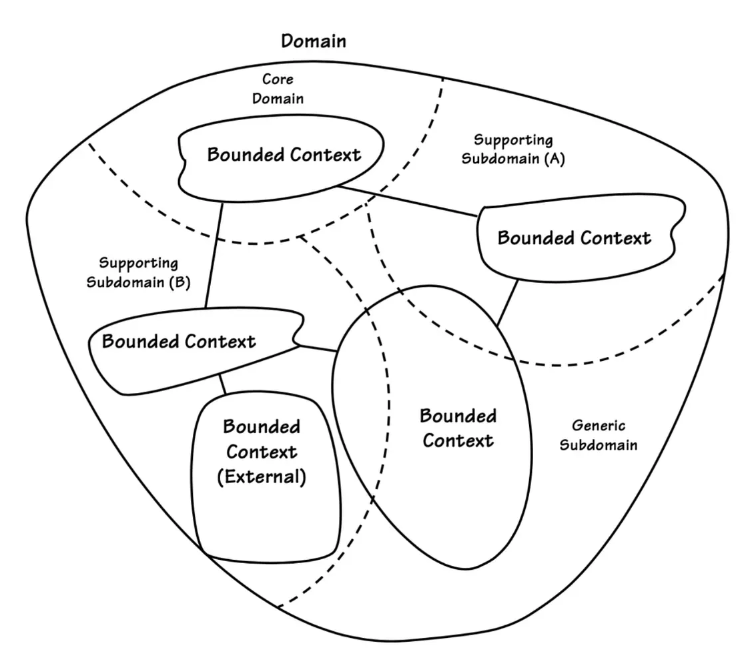
\includegraphics[scale = 0.3]{pictures/333Subdomain.excalidraw.png}
\caption[Các loại miền phụ trong Domain Driven Design]{Các loại miền phụ trong Domain Driven Design (Nguồn: \cite{vernon2013implementing})}
\end{figure}

\item \textbf{Chuyên gia miền (Domain Expert):} Người hiểu sâu sắc nhất về quy trình kinh doanh thực tế, làm việc chặt chẽ với đội ngũ phát triển.

\item \textbf{Ngôn ngữ chung (Ubiquitous Language):} Ngôn ngữ thống nhất được sử dụng xuyên suốt bởi cả đội ngũ kỹ thuật và chuyên gia miền, từ giao tiếp hàng ngày đến việc đặt tên trong mã nguồn.

\item \textbf{Bối cảnh bị giới hạn (Bounded Context):} Xác định ranh giới rõ ràng cho một phần của hệ thống, giúp các nhóm hoạt động độc lập và giữ cho mô hình nhất quán trong phạm vi đó.

\item \textbf{Bản đồ bối cảnh (Context Maps) và Các mối quan hệ:} Thể hiện trực quan cách các Bounded Context giao tiếp với nhau.
\end{itemize}

\vspace{0.5em}
\textbf{Các mẫu kỹ thuật (Tactical Patterns)}

Nhóm mẫu này đóng vai trò hiện thực hóa các khái niệm nghiệp vụ vào thiết kế mã nguồn hệ thống.

\begin{itemize}
\item \textbf{Đối tượng thực thể (Entities Objects):} Các đối tượng có \textbf{định danh duy nhất} (ID) tồn tại xuyên suốt vòng đời.

\item \textbf{Đối tượng giá trị (Value Objects):} Các đối tượng không có định danh duy nhất, dùng để đại diện cho một đặc điểm (ví dụ: địa chỉ, giá tiền). Chúng được so sánh qua các thuộc tính và thường được thiết kế ở dạng bất biến (immutable).

\item \textbf{Tổng hợp (Aggregates):} Một nhóm các thực thể và đối tượng giá trị được gom lại thành một khối thống nhất để đảm bảo tính toàn vẹn dữ liệu. Giao tiếp với bên ngoài bắt buộc phải thông qua một thực thể gốc (Aggregate Root).

\item \textbf{Nhà máy (Factory):} Đóng gói quy trình khởi tạo phức tạp của các đối tượng hoặc Aggregates để đảm bảo chúng luôn được tạo ra ở trạng thái hợp lệ.

\item \textbf{Kho lưu trữ (Repository):} Trừu tượng hóa lớp tương tác với CSDL. Nó hoạt động như một bộ sưu tập lưu trữ các đối tượng Aggregates trong bộ nhớ, giúp mô hình miền tách biệt hoàn toàn khỏi công nghệ lưu trữ.

\item \textbf{Dịch vụ miền (Domain Service):} Nơi chứa các quy tắc hoặc hành vi nghiệp vụ phức tạp liên quan đến nhiều đối tượng, không phù hợp để đặt vào bên trong một thực thể hay đối tượng giá trị cụ thể.
\end{itemize}

\vspace{0.5em}
\textbf{Kiến trúc hệ thống trong DDD}

Để bảo vệ lớp miền cốt lõi khỏi các công nghệ bên ngoài,
dự án áp dụng các kiến trúc lục giác:

\begin{itemize}
% \item \textbf{Kiến trúc phân lớp (Layered Architecture):} Thường chia làm 4 lớp cơ bản: Giao diện người dùng (User Interface) $\rightarrow$ Ứng dụng (Application) $\rightarrow$ Lớp Miền (Domain - trung tâm) $\rightarrow$ Hạ tầng (Infrastructure).

\item \textbf{Kiến trúc lục giác (Hexagonal Architecture / Ports and Adapters):} Đây là kiến trúc được áp dụng chính. Đặt lớp miền (Domain) ở vị trí trung tâm, cách ly hoàn toàn với các yếu tố bên ngoài. Mọi giao tiếp với CSDL, API, hoặc giao diện đều thông qua các \textbf{Cổng (Ports)} và \textbf{Bộ điều hợp (Adapters)}. Kiến trúc này giúp hệ thống cực kỳ dễ kiểm thử, linh hoạt thay đổi công nghệ (Database, Framework) mà không làm ảnh hưởng đến logic nghiệp vụ cốt lõi.

\item \textbf{Nguyên tắc đảo ngược phụ thuộc (Dependency Inversion):} Đảo ngược phụ thuộc là nguyên tắc cốt lõi giúp bảo vệ và cô lập lớp miền (Domain Layer). Cơ chế hoạt động: Lớp Miền sẽ định nghĩa các giao diện (chính là các Cổng - Ports trong kiến trúc lục giác) để yêu cầu những gì nó cần. Các module cấp thấp (như CSDL, hàng đợi tin nhắn) sẽ triển khai các giao diện này (đóng vai trò là Bộ điều hợp - Adapters) và cắm vào lớp Miền như những \enquote{plugin} độc lập.
\end{itemize}

\begin{figure}[H]
\centering
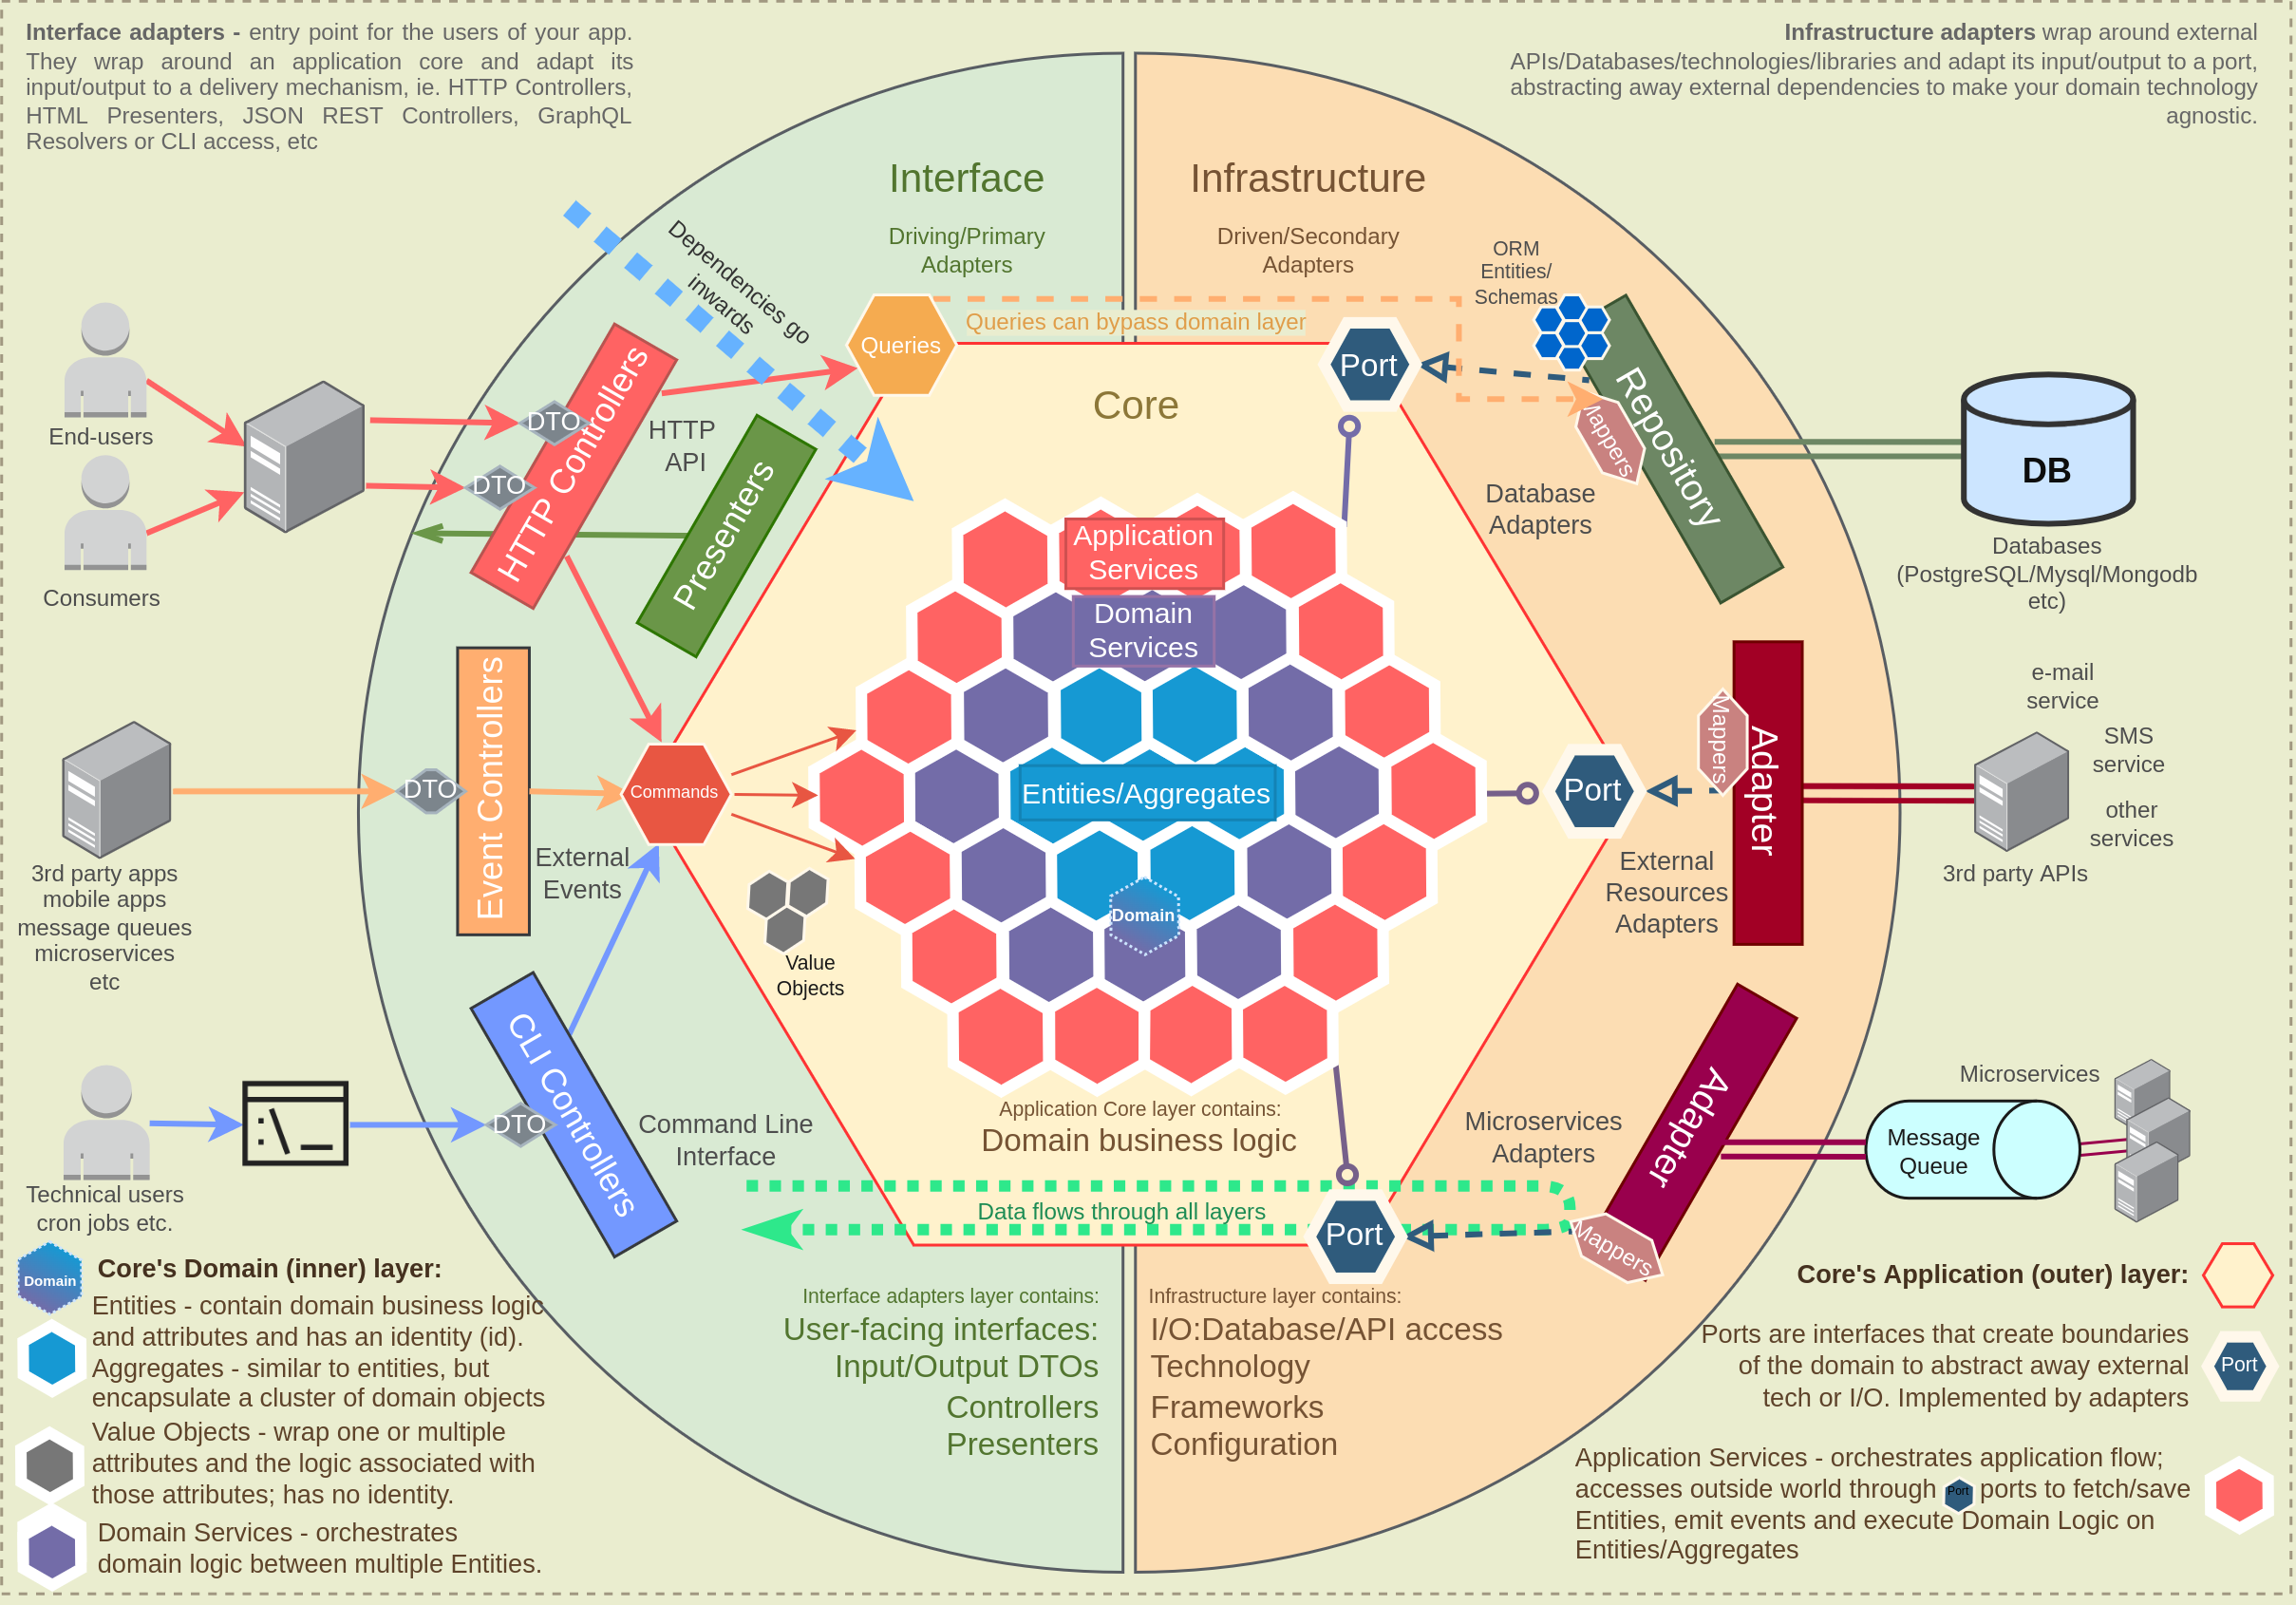
\includegraphics[width=0.6\textwidth]{pictures/DomainDrivenHexagon.png}
\caption[Tổng quan kiến trúc lục giác]{Tổng quan kiến trúc lục giác (Nguồn: \cite{ddd-hexagon})}
\end{figure}

\begin{figure}[H]
\centering
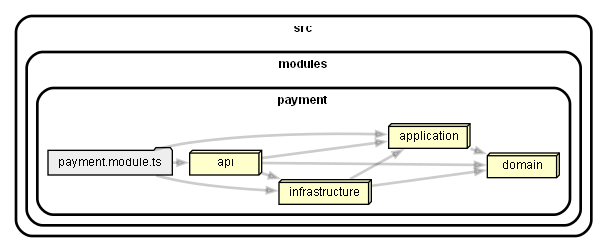
\includegraphics[width=0.6\textwidth]{pictures/architecture-summary-code-payment-service.png}
\caption{Dịch vụ thanh toán áp dụng Domain Driven Design (tạo tự động từ depcruise)}
\end{figure}

\begin{figure}[H]
\centering
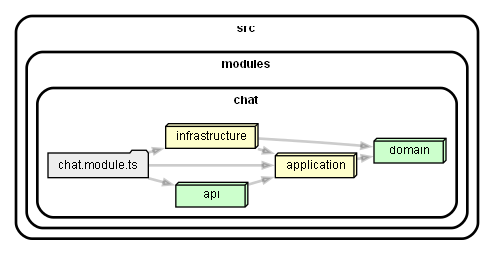
\includegraphics[width=0.6\textwidth]{pictures/architecture-summary-code-conversation-service.png}
\caption{Dịch vụ trò chuyện áp dụng Domain Driven Design (tạo tự động từ depcruise)}
\end{figure}
